\section{Результаты измерений}
Сначала проведём демонстрационный эксперимент.
Из его результатов можно сделать выводы:
\begin{enumerate}
    \item Измеряемая величина флуктуирует
    \item Среднее значение сначала сильно меняется,
    потом выходит на постоянное значение.
    \item Погрешность отдельного измерения тоже
    устанавливается со временем
    \item Средняя погрешность и её колебания со временем уменьшаются
\end{enumerate}

Проведём основной эксперимент, результаты для $t=20\,\text{с}$ занесём
в таблицу \ref{table:1}, а для\\ $t=10\,\text{с}$~--- в таблицу \ref{table:3}.
Разобьём значения из таблицы \ref{table:1} по парам и занесём их суммы в
таблицу~\ref{table:2}.

По данным таблиц~\ref{table:3} и~\ref{table:2} строим гистрограммы.
Светлая гистрограмма построена по таблице~\ref{table:3}, а тёмная~---
по таблице~\ref{table:2}. Масштаб светлой гистрограммы по оси $x$ 
на верхней шкале, тёмной~--- на нижней.

Средние значения чисел срабатывания за $10$ и $40\,\text{с}$:
\begin{displaymath}
\begin{split}
    \overline{n_{10}}\approx 12{,}42 \\
    \overline{n_{40}}\approx 49{,}63
\end{split}
\end{displaymath}

Стандартные отклонения:
\begin{displaymath}
\begin{split}
    \sigma_{n_{10}}\approx 3{,}68 \\
    \sigma_{n_{40}}\approx 7{,}9
\end{split}
\end{displaymath}

Стандартные отклонения не сильно отличяются от $\sqrt{\overline{n}}$:
\begin{displaymath}
\begin{split}
    \sqrt{\overline{n_{10}}}\approx 3{,}52\approx \sigma_{n_{10}} \\
    \sqrt{\overline{n_{40}}}\approx 7{,}04\approx \sigma_{n_{40}}
\end{split}
\end{displaymath}

С увеличением $t$ уменьшается ширина пика и его высота.

Относительная полуширина распределений:
\begin{displaymath}
\begin{split}
    \frac{\sigma_{n_{10}}}{\overline{n_{10}}}\approx 0{,}3 \\
    \frac{\sigma_{n_{40}}}{\overline{n_{40}}}\approx 0{,}16
\end{split}
\end{displaymath}

Стандартная ошибка для $400$ измерений по $10\,\text{с}$ и
для $100$ измерений по $40\,\text{с}$:
\begin{displaymath}
\begin{split}
    \sigma_{\overline{n_{10}}}=\frac{\sigma_{n_{10}}}{\sqrt{400}}\approx 0{,}18 \\
    \sigma_{\overline{n_{40}}}=\frac{\sigma_{n_{40}}}{\sqrt{100}}\approx 0{,}79
\end{split}
\end{displaymath}

Относительные ошибки:
\begin{displaymath}
\begin{split}
    \varepsilon_{\overline{n_{10}}_1} = \frac{\sigma_{\overline{n_{10}}}}{\overline{n_{10}}}\approx 0{,}014 \\
    \varepsilon_{\overline{n_{10}}_2} = \frac{1}{\sqrt{\overline{n_{10}\cdot 400}}}\approx 0{,}014 \\
    \varepsilon_{\overline{n_{40}}_1} = \frac{\sigma_{\overline{n_{40}}}}{\overline{n_{40}}}\approx 0{,}016 \\
    \varepsilon_{\overline{n_{40}}_2} = \frac{1}{\sqrt{\overline{n_{40}\cdot 100}}}\approx 0{,}014
\end{split}
\end{displaymath}

Итого:
\begin{displaymath}
\begin{split}
    n_{10}=12{.}42\pm 0{,}18 \\
    n_{40}=49{.}63\pm 0{,}79
\end{split}
\end{displaymath}

\begin{table}
    \centering
    \caption{Число срабатывания счётчика за 20 секунд}
    \begin{tabular}{|c|c|c|c|c|c|c|c|c|c|c|}
    \hline
        № опыта & 1 & 2 & 3 & 4 & 5 & 6 & 7 & 8 & 9 & 10 \\ \hline
        0 & 39 & 24 & 23 & 30 & 33 & 19 & 24 & 19 & 25 & 22 \\ \hline
        10 & 22 & 29 & 30 & 26 & 13 & 25 & 23 & 19 & 20 & 36 \\ \hline
        20 & 27 & 20 & 34 & 31 & 27 & 21 & 34 & 16 & 21 & 23 \\ \hline
        30 & 29 & 24 & 22 & 26 & 23 & 31 & 26 & 23 & 22 & 11 \\ \hline
        40 & 14 & 21 & 23 & 22 & 21 & 17 & 24 & 30 & 29 & 25 \\ \hline
        50 & 23 & 29 & 22 & 40 & 28 & 29 & 32 & 28 & 20 & 19 \\ \hline
        60 & 18 & 29 & 34 & 26 & 32 & 25 & 17 & 28 & 35 & 21 \\ \hline
        70 & 21 & 25 & 30 & 22 & 23 & 21 & 26 & 17 & 20 & 19 \\ \hline
        80 & 27 & 21 & 24 & 27 & 20 & 28 & 19 & 29 & 25 & 22 \\ \hline
        90 & 30 & 33 & 20 & 18 & 24 & 16 & 21 & 18 & 26 & 24 \\ \hline
        100 & 16 & 38 & 27 & 34 & 18 & 23 & 32 & 21 & 27 & 22 \\ \hline
        110 & 31 & 25 & 23 & 23 & 21 & 21 & 27 & 29 & 31 & 24 \\ \hline
        120 & 28 & 23 & 24 & 28 & 26 & 35 & 27 & 29 & 21 & 28 \\ \hline
        130 & 22 & 21 & 23 & 35 & 31 & 27 & 18 & 18 & 26 & 20 \\ \hline
        140 & 21 & 21 & 23 & 23 & 29 & 37 & 23 & 34 & 37 & 32 \\ \hline
        150 & 23 & 17 & 24 & 25 & 35 & 18 & 23 & 24 & 21 & 23 \\ \hline
        160 & 28 & 20 & 19 & 21 & 14 & 21 & 22 & 24 & 21 & 24 \\ \hline
        170 & 31 & 14 & 26 & 28 & 23 & 34 & 24 & 19 & 18 & 20 \\ \hline
        180 & 32 & 24 & 29 & 26 & 24 & 23 & 20 & 26 & 29 & 40 \\ \hline
        190 & 16 & 20 & 26 & 31 & 25 & 34 & 23 & 27 & 21 & 31 \\ \hline
    \end{tabular}
    \label{table:1}
\end{table}

\begin{table}
    \centering
    \caption{Число срабатывания счётчика за 40 секунд}
    \begin{tabular}{|c|c|c|c|c|c|c|c|c|c|c|}
    \hline
        № опыта & 1 & 2 & 3 & 4 & 5 & 6 & 7 & 8 & 9 & 10 \\ \hline
        0 & 63 & 53 & 52 & 43 & 47 & 51 & 56 & 38 & 42 & 56 \\ \hline
        10 & 47 & 65 & 48 & 50 & 44 & 53 & 48 & 54 & 49 & 33 \\ \hline
        20 & 35 & 45 & 38 & 54 & 54 & 52 & 62 & 57 & 60 & 39 \\ \hline
        30 & 47 & 60 & 57 & 45 & 56 & 46 & 52 & 44 & 43 & 39 \\ \hline
        40 & 48 & 51 & 48 & 48 & 47 & 63 & 38 & 40 & 39 & 50 \\ \hline
        50 & 54 & 61 & 41 & 53 & 49 & 56 & 46 & 42 & 56 & 55 \\ \hline
        60 & 51 & 52 & 61 & 56 & 49 & 43 & 58 & 58 & 36 & 46 \\ \hline
        70 & 42 & 46 & 66 & 57 & 69 & 40 & 49 & 53 & 47 & 44 \\ \hline
        80 & 48 & 40 & 35 & 46 & 45 & 45 & 54 & 57 & 43 & 38 \\ \hline
        90 & 56 & 55 & 47 & 46 & 69 & 36 & 57 & 59 & 50 & 52 \\ \hline
    \end{tabular}
    \label{table:2}
\end{table}

\begin{table}
    \centering
    \caption{Число срабатывания счётчика за 10 секунд}
    \begin{tabular}{|c|c|c|}
    \hline
        Число импульсов & Число случаев & Доля случаев \\ \hline
        4 & 2 & 0.005 \\ \hline
        5 & 1 & 0.0025 \\ \hline
        6 & 13 & 0.0325 \\ \hline
        7 & 14 & 0.035 \\ \hline
        8 & 26 & 0.065 \\ \hline
        9 & 31 & 0.0775 \\ \hline
        10 & 43 & 0.1075 \\ \hline
        11 & 46 & 0.115 \\ \hline
        12 & 40 & 0.1 \\ \hline
        13 & 46 & 0.115 \\ \hline
        14 & 30 & 0.075 \\ \hline
        15 & 26 & 0.065 \\ \hline
        16 & 23 & 0.0575 \\ \hline
        17 & 26 & 0.065 \\ \hline
        18 & 11 & 0.0275 \\ \hline
        19 & 6 & 0.015 \\ \hline
        20 & 6 & 0.015 \\ \hline
        21 & 3 & 0.0075 \\ \hline
        22 & 3 & 0.0075 \\ \hline
        23 & 2 & 0.005 \\ \hline
        24 & 1 & 0.0025 \\ \hline
        25 & 1 & 0.0025 \\ \hline
    \end{tabular}
    \label{table:3}
\end{table}

\begin{figure}
    \centering
    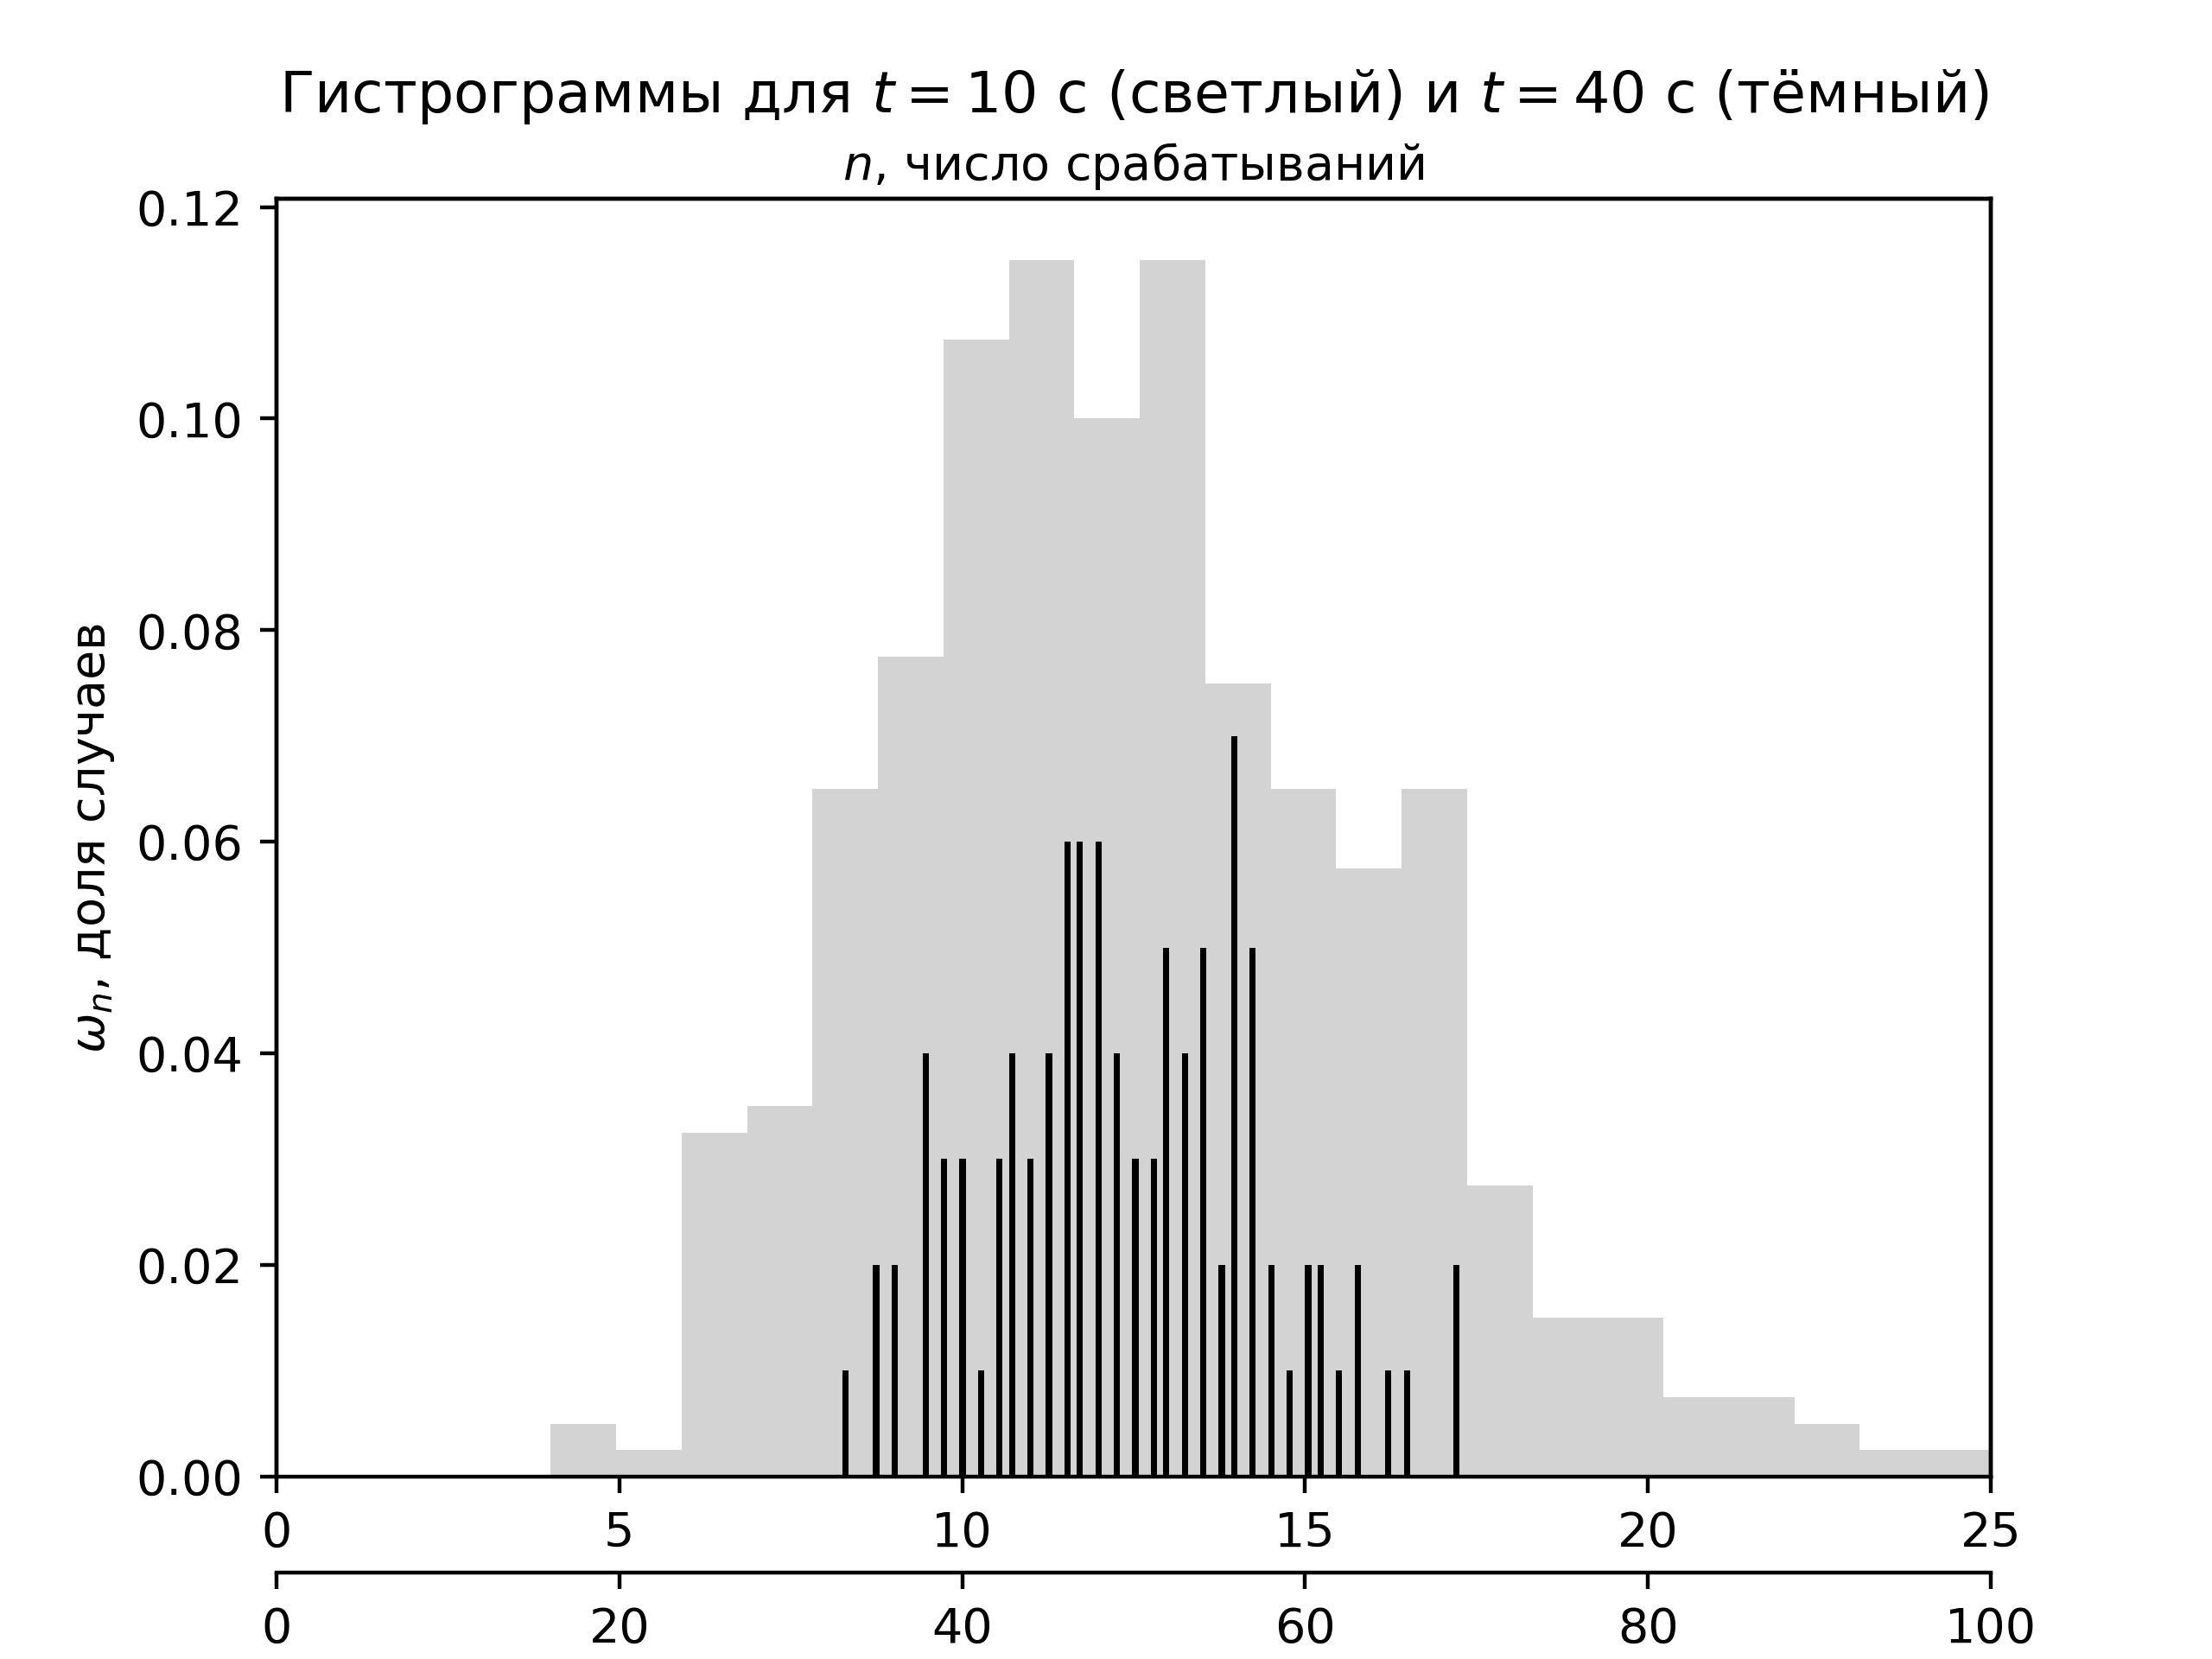
\includegraphics{jupiter/lol.png}
\end{figure}

\begin{table}
    \centering
    \caption{Доля отклонений}
    \begin{tabular}{|l|c|c|}
    \hline
    Ошибка                 & Доля случаев & Теоретическая оценка \\ \hline
    $\pm\sigma_{n_{10}}$   & 0.71         & 0.68                 \\ \hline
    $\pm 2\sigma_{n_{10}}$ & 0.95         & 0.95                 \\ \hline
    $\pm\sigma_{n_{40}}$   & 0.7          & 0.68                 \\ \hline
    $\pm 2\sigma_{n_{40}}$ & 0.96         & 0.95                 \\ \hline
    \end{tabular}
    \label{table:4}
\end{table}

\newpage
~
\newpage

\section{Вывод}
Получены данные интенсивности радиоактивного фона, применены методы экспериментальной обработки данных.
